\documentclass[12pt,a4paper]{article}
\usepackage{mainsty}
\begin{document}

\begin{center}
  \large\textsc{\imp{Induction \& Recursion}}
\end{center}
\begin{enumerate}
  \item \textbf{Sequences} is a special type of function in which the domain is a set of consecutive integers.
  A geometric sequence is a sequence of real numbers where each term after the initial term is found by taking the previous term and multiplying by a fixed number called the common ratio. A geometric sequence can be finite or infinite.
  \item \textbf{Recurrence relations} Some sequences are most naturally defined by specifying one or more initial terms and then giving a rule for determining subsequent terms from earlier terms in the sequence. A rule that defines a term an as a function of previous terms in the sequence is called a recurrence relation.
  \item \textbf{Summations}
  \begin{itemize}
    \item 
  \end{itemize}
  \item \textbf{Mathematical induction} The \textbf{base case} establishes that the theorem is true for the first value in the sequence.
  The \textbf{inductive step} establishes that if the theorem is true for k, then the theorem also holds for k + 1
  \begin{itemize}
    \item 
  \end{itemize}
  \item \textbf{Strong induction and well-ordering} The principle of strong induction assumes that the fact to be proven holds for all values less than or equal to k and proves that the fact holds for k+1. By contrast the standard form of induction only assumes that the fact holds for k in proving that it holds for k+1.
  \item \textbf{Loop invariants} The field of \textbf{program verification} is concerned with formally proving that programs perform correctly. A program's correct behavior is defined by stating that if a \textbf{pre-condition} is true before the program starts, then the program will end after a finite number of steps and a \textbf{post-condition} is true after the program ends.
  \item \textbf{Recursive definitions} In a \textbf{recursive definition} of a function, the value of the function is defined in terms of the output value of the function on smaller input values. One can use the recursive definition for n! to determine the value of the factorial function on a particular value for n by starting at 0, multiplying 0! by 1 to get the value of 1! then multiplying by 2 to get 2!, and so on, until the desired n! has been reached. The process is called recursion. \textbf{Recursion} is the process of computing the value of a function using the result of the function on smaller input values.
  \item \textbf{Structural induction} is a type of induction used to prove theorems about recursively defined sets that follows the structure of the recursive definition.
  \item \textbf{Recursive algorithms}
  \begin{itemize}
    \item 
  \end{itemize}
  \item \textbf{Induction and recursive algorithms}
  \begin{itemize}
    \item 
  \end{itemize}
  \item \textbf{Analyzing the time complexity of recursive algorithms}
  \begin{itemize}
    \item 
  \end{itemize}
  \item \textbf{Divide-and-conquer algorithms: Introduction and mergesort}
  \begin{itemize}
    \item 
  \end{itemize}
  \item \textbf{Divide-and-conquer algorithms: Binary search}
  \begin{itemize}
    \item 
  \end{itemize}
  \item \textbf{Solving linear homogeneous recurrence relations}
  \begin{itemize}
    \item 
  \end{itemize}
  \item \textbf{Solving linear non-homogeneous recurrence relations}
  \begin{itemize}
    \item 
  \end{itemize}
  \item \textbf{Divide-and-conquer recurrence relations}
  \begin{itemize}
    \item 
  \end{itemize}
\end{enumerate}


\clearpage
\begin{center}
  \large\textsc{\imp{Integer Properties}}
\end{center}
\begin{enumerate}
  \item \textbf{The Division Algorithm}
  \begin{itemize}
    \item \textbf{Integer division}
  \end{itemize}
  \item \textbf{Modular arithmetic} 
  \begin{itemize}
    \item \textbf{Modular arithmetic}
  \end{itemize}
  \item \textbf{Prime factorizations}
  \begin{itemize}
    \item \textbf{prime}
    \item \textbf{composite}
    \item \textbf{prime factorization}
    \item \textbf{non-decreasing}
    \item \textbf{multiplicity}
  \end{itemize}
  \item \textbf{Factoring and primality testing}
  \item \textbf{Greatest common divisor and Euclid's algorithm}
  \begin{itemize}
    \item \textbf{GCD Theorem}
    \item \textbf{Euclid's algorithm for finding the greatest common divisor}
    \item \textbf{The extended Euclidean algorithm}
  \end{itemize}
  \item \textbf{Number representation}
  \begin{itemize}
    \item A digit in binary notation is called a \textbf{bit}. Numbers represented in \textbf{base} b require b distinct symbols and each place value is a power of b.
  \end{itemize}
  \item \textbf{Fast exponentiation}
  \begin{itemize}
    \item Computing a power of x by repeated multiplication by x
    \item Computing a power of x by repeated squaring
  \end{itemize}
  \item \textbf{The RSA cryptosystem}
  \begin{itemize}
    \item In \textbf{public key cryptography}, Bob has an \textbf{encryption key} that he provides publicly so that anyone can use it to send him an encrypted message. Bob holds a matching \textbf{decryption key} that he keeps privately to decrypt messages. While anyone can use the public key to encrypt a message, the security of the scheme depends on the fact that it is difficult to decrypt the message without having the matching private decryption key. 
    \item Encryption
    \item Decryption
  \end{itemize}
\end{enumerate}


\clearpage
\begin{center}
  \large\textsc{\imp{Intro to Counting}}
\end{center}
\begin{enumerate}
  \item \textbf{Sum and product rules}
  \begin{itemize}
    \item \textbf{Product Rule}
    \item \textbf{Sum Rule}
  \end{itemize}
  \item \textbf{The bijection rule}
  \begin{itemize}
    \item \textbf{Bijection Rule}
  \end{itemize}
  \item \textbf{The generalized product rule}
  \begin{itemize}
    \item \textbf{Generalized Product Rule}
  \end{itemize}
  \item \textbf{Counting permutations}
  \begin{itemize}
    \item \textbf{Permutation}
  \end{itemize}
  \item \textbf{Counting subsets}
  \begin{itemize}
    \item \textbf{Subset}
    \item \textbf{r-combination}
  \end{itemize}
  \item \textbf{Counting by complement}
  \begin{itemize}
    \item \textbf{Counting by complement}
  \end{itemize}
  \item \textbf{Permutations with repetitions}
  \begin{itemize}
    \item \textbf{Permutation with repetition}
  \end{itemize}
  \item \textbf{Counting multisets}
  \begin{itemize}
    \item \textbf{Multisets}
  \end{itemize}
  \item \textbf{Inclusion-exclusion principle}
  \begin{itemize}
    \item \textbf{Principle of inclusion-exclusion}
  \end{itemize}
\end{enumerate}


\clearpage
\begin{center}
  \large\textsc{\imp{Graphs}}
\end{center}
\begin{enumerate}
  \item \textbf{Introduction to graphs} Directed graphs were introduced in the context of relations. Here we are concerned with \textbf{undirected graphs}. In an undirected graph, the edges are unordered pairs of vertices, which is useful for modeling relationships that are symmetric.
  A graph consists of a pair of sets (V, E), where V is a set of vertices and E is a set of edges. A graph is \textbf{finite} if the vertex set is finite. This material will only be concerned with finite graphs. A single element of V is called a \textbf{vertex} and is usually represented pictorially by a dot with a label. Each edge in E is a set of two vertices from V and is drawn as a line connecting the two vertices. In the graph below, the vertex set is V = \{a, b, c, d, e\}. The graph has six edges.
  \textbf{Parallel edges} are multiple edges between the same pair of vertices. Imagine a graph whose vertex set is a set of cities and whose edges are roads connecting pairs of cities. It is possible for there to be two different roads between the same two cities. In defining graphs with parallel edges, it would be important to have an additional label besides the two endpoints to specify an edge in order to distinguish between different parallel edges. A graph can also have a \textbf{self-loop} which is an edge between a vertex and itself. The graph below has two parallel edges between vertices a and b. There is also a self-loop at vertex c.
  \begin{itemize}
    \item[] 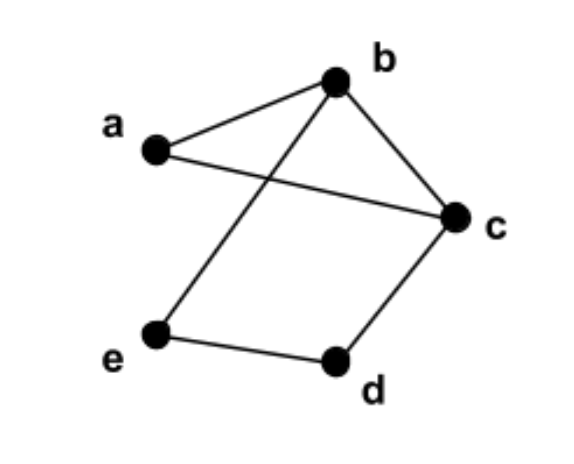
\includegraphics{graph}
    \item If there is an edge between two vertices, they are said to be \textbf{adjacent}. In the graph above, d and e are adjacent, but d and b are not adjacent.
    \item Vertices b and e are the \textbf{endpoints} of edge \{b, e\}. The edge \{b, e\} is \textbf{incident} to vertices b and e.
    \item A vertex c is a \textbf{neighbor} of vertex b if and only if \{b, c\} is an edge. In the graph above, the neighbors of b are the vertices a, c, and e.
    \item In a simple graph, the \textbf{degree} of a vertex is the number of neighbors it has. In the graph above, the degree of b is 3 and the degree of vertex a is 2. The degree of vertex b is denoted by deg (b).
    \item The \textbf{total degree} of a graph is the sum of the degrees of all of the vertices. The total degree of the graph above is 2 + 3 + 3 + 2 + 2 = 12.
    \item[] 
  \end{itemize}
  \item \textbf{Graph representations}
  \begin{itemize}
    \item In the \textbf{adjacency list} representation of a graph, each vertex has a list of all its neighbors. Note that since the graph is undirected if vertex a is in b's list of neighbors, then b must also be in a's list of neighbors.
    \item The \textbf{matrix} representation for a graph with n vertices is an n by n matrix whose entries are all either 0 or 1, indicating whether or not each edge is present. If the matrix is labeled M, then \(M_{i,j} \) denotes the entry in row i and column j. For a matrix representation, the vertices of the graph are labeled with integers in the range from 1 to n. Entry \(M_{i,j=1} \) if and only if \{i, j\} is an edge in the graph. Since the graph is undirected, \(M_{i,j} \) = \(M_{j,i} \) because \{i, j\} and \{j, i\} refer to the same edge which is either present in the graph or not. Thus the matrix representation of an undirected graph is symmetric about the diagonal, meaning that it is a mirror image of itself along the diagonal extending from the upper left corner to the lower right corner.
  \end{itemize}
  \item \textbf{Graph isomorphism}: Two graphs are said to be \textbf{isomorphic} if there is a correspondence between the vertex sets of each graph such that there is an edge between two vertices of one graph if and only if there is an edge between the corresponding vertices of the second graph. The graphs are not identical but the vertices can be relabeled so that they are identical.
  \begin{itemize}
    \item Let G = (V, E) and G' = (V',E').  G and G' are isomorphic if there is a bijection f: V → V' such that for every pair of vertices x, y \(\in \) V, \{x, y\} \(\in \) E if and only if \( \{f(x), f(y)\} \) \(\in \) E'. The function f is called an \textbf{isomorphism} from G to G'.
  \end{itemize}
  \item \textbf{Walks, trails, circuits, paths, and cycles}:
  \begin{itemize}
    \item A \textbf{walk} from \(v_0 \) to \(v_l \) in an undirected graph G is a sequence of alternating vertices and edges that starts and ends with a vertex:\\ 
    \(\langle \blu{v_{0}},\red{\{v_{0},v_{1} \}}, \blu{v_{1}}, \red{\{v_{1}, v_{2} \}}, \blu{v_{1},\ldots,v_{l-1}}, \red{\{v_{l-1}, v_{l} \}}, \blu{v_{l}} \rangle \)
    \item The vertices just before and after each edge are the two endpoints of that edge.
    \item Since the edges in a walk are completely determined by the vertices, a walk can also be denoted by the sequence of vertices: \(\langle \blu{v_{0}, v_{1},\ldots, v_{l}} \rangle \)
    \item The sequence of vertices is a walk only if \( \{v_{i-1}, v_i\} \) \(\in \) E for each i = 1, 2,\(\ldots \),l. Two consecutive vertices \(\ldots \), \( v_{i-1}, v_i \), \(\ldots \) in a walk represent an occurrence of the edge \( \{v_{i-1}, v_i\} \) in the walk.
    \item The \textbf{length} of a walk is l, the number of edges in the walk.
    \item An \textbf{open walk} is a walk in which the first and last vertices are not the same. A \textbf{closed walk} is a walk in which the first and last vertices are the same.
    \item A \textbf{trail} is an open walk in which no edge occurs more than once.
    \item A \textbf{circuit} is a closed walk in which no edge occurs more than once.
    \item A \textbf{path} is a trail in which no vertex occurs more than once.
    \item A \textbf{cycle} is a circuit of length at least 1 in which no vertex occurs more than once, except the first and last vertices which are the same.
  \end{itemize}
  \item \textbf{Graph connectivity}: In an undirected graph, if there is a path from vertex v to vertex w, then there is also a path from w to v. The two vertices, v and w, are said to be \textbf{connected}. A vertex is always considered to be connected to itself. If the graph represents a road or communication network, then it is very desirable for every pair of vertices to be connected. The property of being connected can be extended to sets of vertices and the entire graph:
  \begin{itemize}
    \item A set of vertices in a graph is said to be connected if every pair of vertices in the set is connected.
    \item A graph is said to be connected if every pair of vertices in the graph is connected, and is \textbf{disconnected} otherwise.
    \item A \textbf{connected component} is a maximal set of vertices that is connected. The word ``maximal'' means that if any vertex is added to a connected component, then the set of vertices will no longer be connected.
    \item A vertex that is not connected with any other vertex is called an \textbf{isolated vertex} and is therefore a connected component with only one vertex.
    \item An undirected graph G is \textbf{k-vertex-connected} if the graph contains at least k + 1 vertices and remains connected after any k -\ 1 vertices are removed from the graph. The \textbf{vertex connectivity} of a graph is the largest k such that the graph is k-vertex-connected. The vertex connectivity of a graph G is denoted \(k(G)\).
    \item An undirected graph G is \textbf{k-edge-connected} if it remains connected after any k -\ 1 edges are removed from the graph. The \textbf{edge connectivity} of a graph is the largest k such that the graph is k-edge-connected. The edge connectivity of a graph G is denoted \(\lambda (G)\).
  \end{itemize}
  \item \textbf{Euler circuits and trails}
  \begin{itemize}
    \item An \textbf{Euler circuit} in an undirected graph is a circuit that contains every edge and every vertex. Note that a circuit, by definition, has no repeated edges, so an Euler circuit contains each edge exactly once.
    \item If an undirected graph G has an Euler circuit, then G is connected and every vertex in G has an even degree.
    \item If an undirected graph G is connected and every vertex in G has an even degree, then G has an Euler circuit.
    \item An undirected graph G has an Euler circuit if and only if G is connected and every vertex in G has even degree.
    \item An \textbf{Euler trail} is an open trail that includes each edge. Note that a trail, by definition, has no repeated edges, so an Euler trail contains each edge exactly once. In an open trail, the first and last vertices are not equal. As with Euler circuits, there is a simple set of conditions that characterize when an undirected graph has an Euler trail.
    \item An undirected graph G has an Euler trail if and only if G is connected and has exactly two vertices with odd degree.
  \end{itemize}
  \item \textbf{Hamiltonian cycles and paths}
  \begin{itemize}
    \item A \textbf{Hamiltonian cycle} in an undirected graph is a cycle that includes every vertex in the graph. Note that a cycle, by definition, has no repeated vertices or edges, except for the vertex which is at the beginning and end of the cycle. Therefore, every vertex in the graph appears exactly once in a Hamiltonian cycle, except for the vertex which is at the beginning and end of the cycle.
    \item A \textbf{Hamiltonian path} in an undirected graph is a path that includes every vertex in the graph. Note that a path, by definition, has no repeated vertices or edges, so every vertex appears exactly once in a Hamiltonian path.
    \item[] 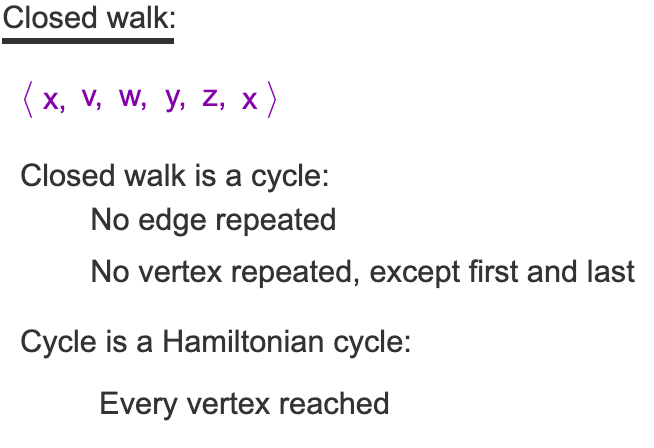
\includegraphics{closed1}
    \item[] 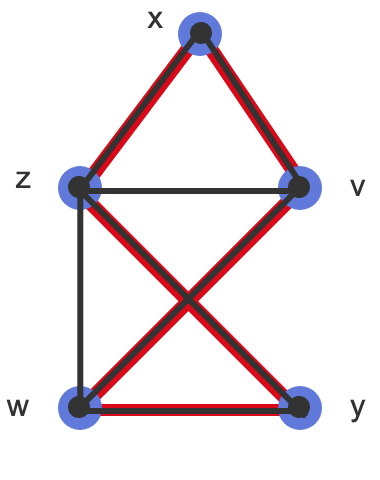
\includegraphics{closed}
    \item[] 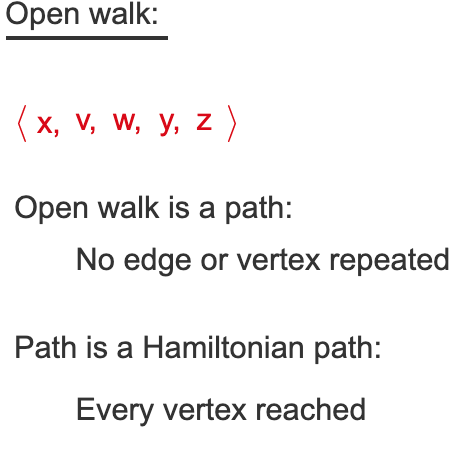
\includegraphics{open1} 
    \item[] 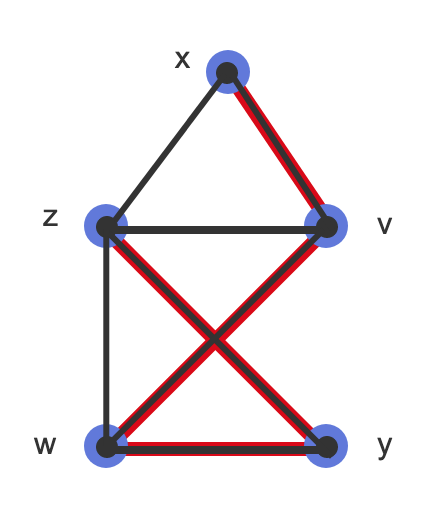
\includegraphics{open}    
  \end{itemize}
  \item \textbf{Planar graphs}
  \begin{itemize}
    \item Graph G\\V = \{ a, b, c, d, e \} \\E = \{ \{ a, b \}, \{ b, c \}, \{ c, d \}, \{ d, a \}, \{ a, c \}, \{ b, d \}, \{ e, a \}, \{ e, b \} \}
    \item[] 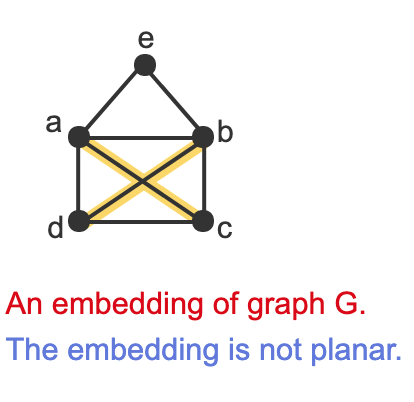
\includegraphics{planar1}
    \item[] 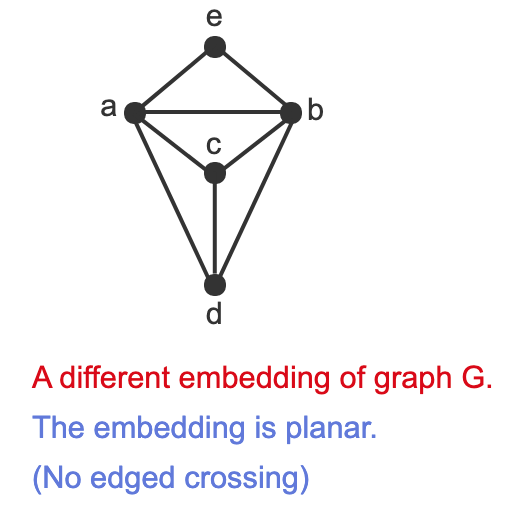
\includegraphics{planar2}
  \end{itemize}
  \item \textbf{Graph coloring}
  \begin{itemize}
    \item Let G = (V, E) be an undirected graph and C a finite set of colors. A \textbf{valid coloring} of G is a function f: V → C such that for every edge \{x, y\} \(\in \) E, \(f(x) \neq f(y)\). If the size of the range of function f is k, then f is called a \textbf{k-coloring} of G.
    \item The \textbf{greedy coloring algorithm}:
    \item Number the set of possible colors. Assume that there is a very large supply of different colors, even though they might not all be used.
    \item Order the vertices in any arbitrary order.
    \item Consider each vertex v in order:
    \begin{itemize}
      \item Assign v a color that is different from the color of v's neighbors that have already been assigned a color. When selecting a color for v, use the lowest numbered color possible.
    \end{itemize}
  \end{itemize}
\end{enumerate}


\clearpage
\begin{center}
  \large\textsc{\imp{Trees}}
\end{center}
\begin{enumerate}
  \item \textbf{Introduction to trees} -\ A \textbf{tree} is an undirected graph that is connected and has no cycles.
  The tree on the left is called a \textbf{free tree} because there is no particular organization of the vertices and edges. The tree on the right is called a \textbf{rooted tree}. The vertex at the top of the drawing is designated as the \textbf{root} of the tree. The remaining vertices are organized according to their distance from the root. The distance between two vertices in an undirected graph is the number of edges in the shortest path between the two vertices. The \textbf{level} of a vertex is its distance from the root. The \textbf{height} of a tree is the highest level of any vertex. The tree on the right has height 3.
  \item[] 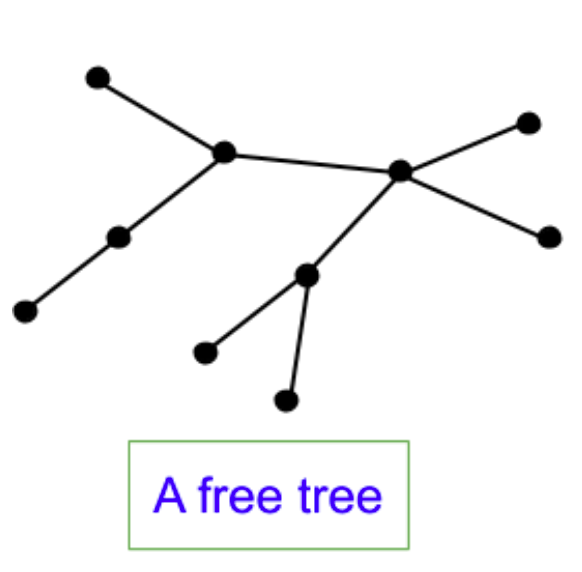
\includegraphics{freetree}
  \item[] 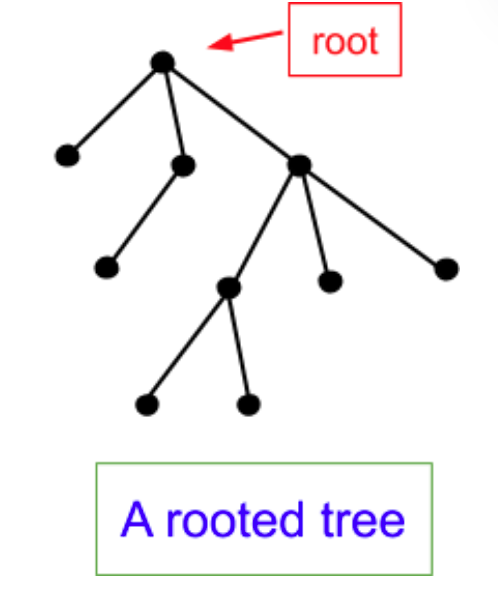
\includegraphics{rootedtree}
  \item[] 
  \item[] 
  \begin{itemize}
    \item[] 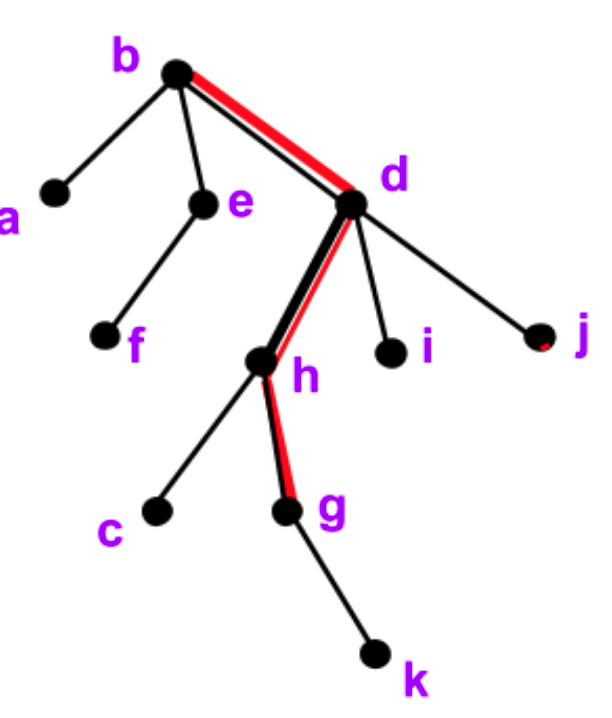
\includegraphics{tree}
    \item Every vertex in a rooted tree T has a unique \textbf{parent}, except for the root which does not have a parent. The parent of vertex v is the first vertex after v encountered along the path from v to the root. (Ex: The parent of vertex g is h.) 
    \item Every vertex along the path from v to the root (except for the vertex v itself) is an ancestor of vertex v. (Ex: The \textbf{ancestors} of vertex g are h, d, and b.)
    \item If v is the parent of vertex u, then u is a \textbf{child} of vertex v. (Ex: Vertices c and g are the children of vertex h.)
    \item If u is an ancestor of v, then v is a \textbf{descendant} of u. (Ex: The descendants of vertex h are c, g, and k.)
    \item A \textbf{leaf} is a vertex which has no children. (Ex: The leaves are a, f, c, k, i, and j.)
    \item Two vertices are \textbf{siblings} if they have the same parent. (Ex: Vertices h, i, and j are siblings because they have the same parent, which is vertex d.)
    \item A \textbf{subtree} rooted at vertex v is the tree consisting of v and all v's descendants. (Ex: The subtree rooted at h includes h, c, g, and k and the edges between them.)
  \end{itemize} 
  \item \textbf{Tree application examples}
  \item \textbf{Properties of trees} -\ The definitions for parent and child vertices in rooted trees make use of the fact that every vertex has a unique path to the root. There is, in fact, a unique path between any pair of vertices in a tree. The theorem below applies to free trees as well as rooted trees.
  \textbf{Theorem}: There is a unique path between every pair of vertices in a tree.
  \begin{itemize}
    \item \textbf{Proof}. A tree is defined to be a connected graph with no cycles. Because every tree is connected, there is at least one path between every pair of vertices. It remains to establish that there is at most one path between every pair of vertices. The proof is by contrapositive. We assume that there is a pair of vertices u and v such that there are two distinct paths between u and v and then show that the graph must have a cycle (and therefore can not be a tree).
    \item[] 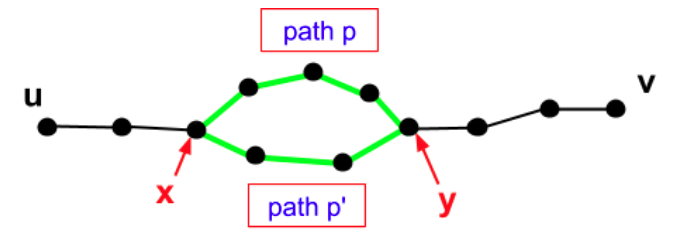
\includegraphics{t1}
    \item Let p and p' be the two distinct paths between u and v. Find the first place where the two paths differ. Let x be the vertex just before the point where the two paths diverge. Follow path p until it hits a vertex y that is also contained in p'. (Both paths end up at v, so there has to be a point where the two paths come together). The portion of the path p between x and y and the portion of the path p' between x and y form a cycle. 
    \item[]
    \item The term leaf is defined in rooted trees as a vertex with no children. A leaf has a natural definition in free trees as well. A leaf of a free tree is a vertex of degree 1. There is one technicality: if a free tree has only one vertex, then that vertex is a leaf. A vertex is an internal vertex if the vertex has degree at least two. The following theorem gives a lower bound on the number of leaves in a free tree:
    \item[] \textbf{Theorem}: Any free tree with at least two vertices has at least two leaves.
    \item \textbf{Proof}. Find the longest path p in the tree. Let u and v be the first and last vertices in the path. Suppose u is not a degree 1 vertex. (The same argument will hold for v). Then there is an edge e that is incident to u and not part of the path p.
    \item[] 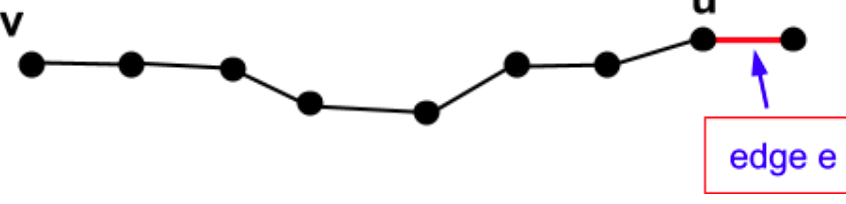
\includegraphics{t2}
    \item If the other endpoint of e, that is not vertex u, is part of the path p, then the graph has a cycle and is not a tree. The path p can be extended by adding e along with the other endpoint of e. The fact that the path p can be extended contradicts the assumption that p was the longest path in the tree.
    \item \textbf{Theorem}: Let T be a tree with n vertices and m edges, then m = n -\ 1
    \item \textbf{Proof}. The proof is by induction on the number of vertices. The base case is where n = 1. If T has one vertex, then it is has no edges. Then m = 0 = n -\ 1.
    \item For the inductive step, assume the theorem holds for trees with n -\ 1 vertices and prove that it holds for trees with n vertices. Consider an arbitrary tree T with n vertices. Since n \(\leq \) 2, by the previous theorem, the tree has at least two leaves. Let v be one of the leaves. Remove v from T along with the edge e incident to v. The resulting graph (call it T') is also a tree and has n-1 vertices.
    \item[] 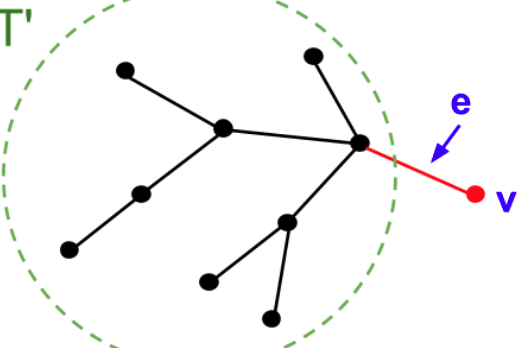
\includegraphics{t3}
    \item By the induction hypothesis, The number of edges in T' is (n -\ 1) -\ 1 = n -\ 2. T has exactly one more edge than T', because only edge e was removed from T to get T'. Therefore the number of edges in T is n -\ 2 + 1 = n -\ 1 
  \end{itemize}
  \item \textbf{Tree traversals}
  \begin{itemize}
    \item Pseudocode for pre-order traversal.
    \item[] 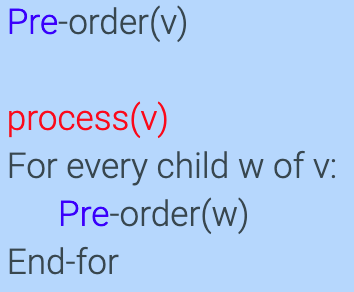
\includegraphics{pre}
    \item[] 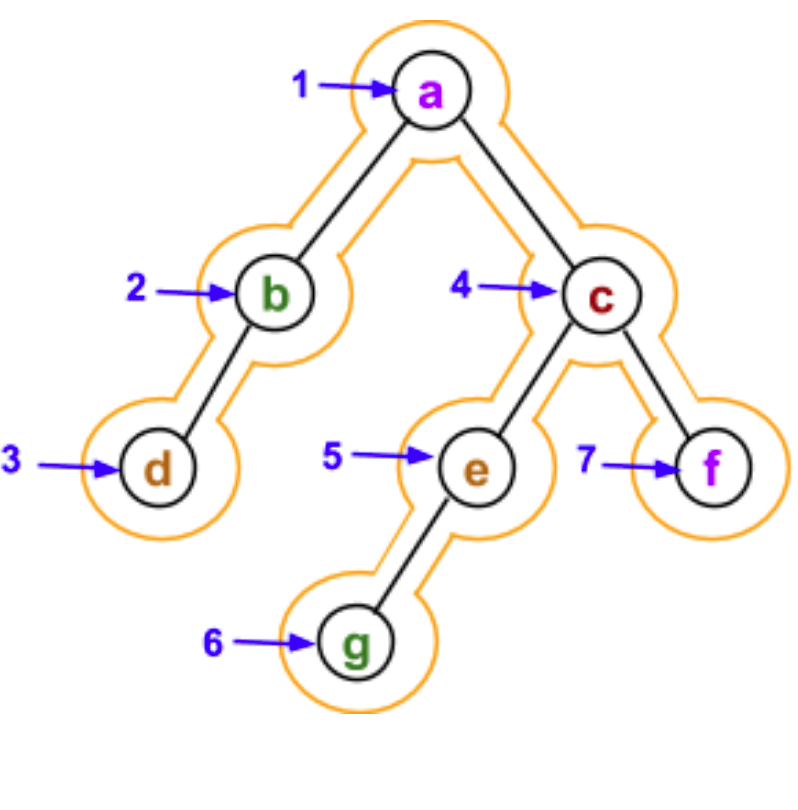
\includegraphics{pre1} 
    \item[] 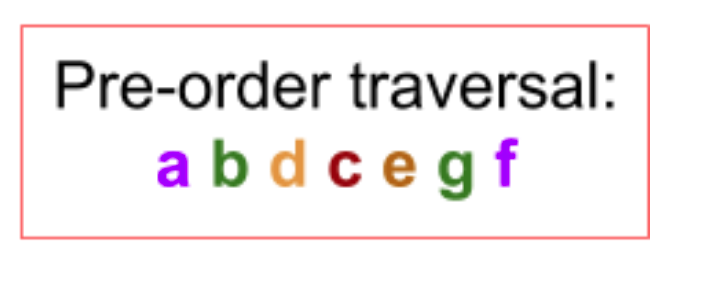
\includegraphics{pre2} 
    \item Pseudocode for post-order traversal.
    \item[] 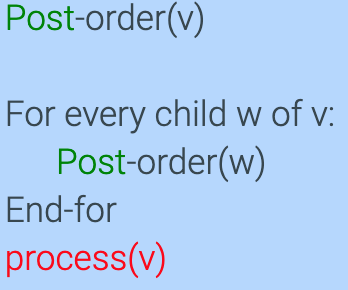
\includegraphics{post}
    \item[] 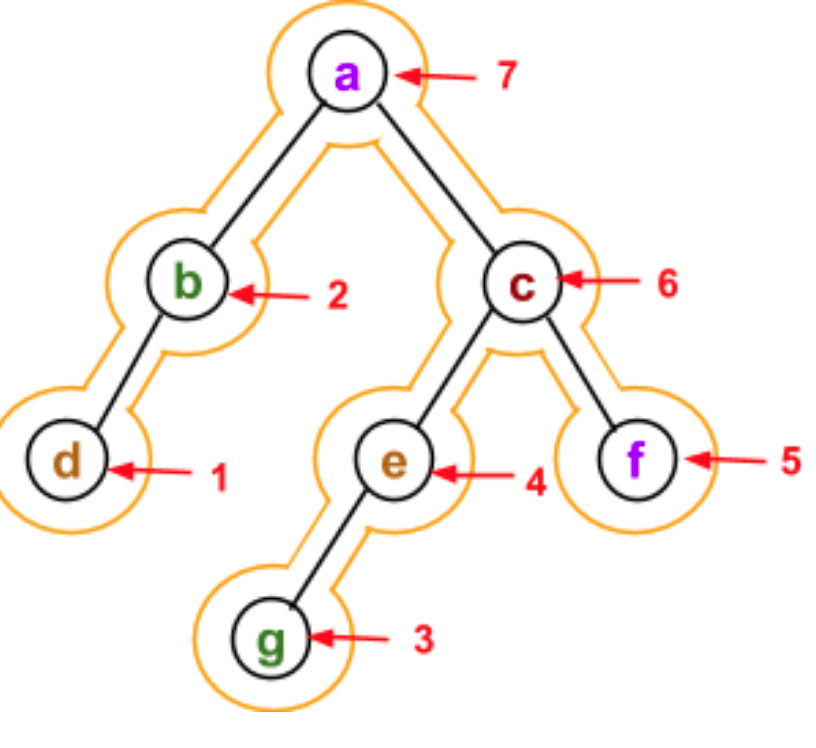
\includegraphics{post1}
    \item[] 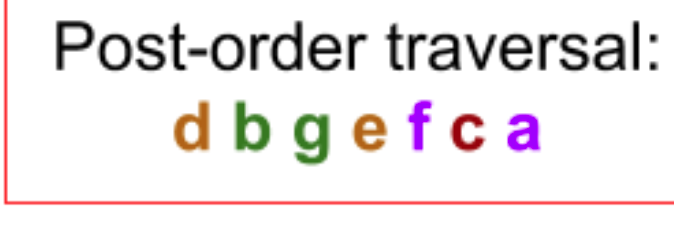
\includegraphics{post2} 
  \end{itemize}
  \item \textbf{Spanning trees and graph traversals}
  \begin{itemize}
    \item A spanning tree of a connected graph G is a subgraph of G which contains all the vertices in G and is a tree.
    \item \textbf{Depth-First Search}
    \item[]
    \item \textbf{Breadth-first-search}
    \item[]   
  \end{itemize}
  \item \textbf{Minimum spanning trees}: A spanning tree of a graph specifies a subset of the edges that provides connectivity between every pair of vertices while minimizing the number of edges included. Every spanning tree of a graph with n nodes has n-1 edges, so there is no reason to prefer one spanning tree over another if the only goal is to include as few edges as possible.
  \begin{itemize}
    \item A \textbf{weighted graph} is a graph G = (V, E), along with a function w: E → R. The function w assigns a real number to every edge.
    \item A \textbf{minimum spanning tree (MST)} of a weighted graph, is a spanning tree T of G whose weight is no larger than any other spanning tree of G.
    \item A graph can have more than one minimum spanning tree because there can be more than one spanning tree with the same weight. In the extreme case, if the weight of every edge is 1, then every spanning tree has weight n -\ 1 and every spanning tree is also a minimum spanning tree.
    \item \textbf{Prim's algorithm} finds a minimum spanning tree
  \end{itemize}
\end{enumerate}
\end{document}